\section{Langkah-Langkah Percobaan}
Pada modul P2 ini, praktikan melakukan \textbf{Routing \& Manajemen IPv6} dengan percobaan untuk melakukan \textbf{routing statis dan dinamis} pada IPv6.

\subsection{Routing Statis}
Dalam routing statis, langkah-langkah yang dilakukan adalah sebagai berikut:
\begin{enumerate}
    \item Mempersiapkan alat dan bahan yang dibutuhkan.
    \item Menghubungkan router dan laptop sesuai skema topologi yang ada pada modul.
    \item Mengkonfigurasikan router masing-masing.
    \item Mereset router untuk menghapus konfigurasi yang ada.
    \item Login ke router menggunakan Winbox, kemudian konfigurasi IP address pada interface router:
    \begin{itemize}
        \item IP \texttt{ether1} Router A: \texttt{2001:db8:1::1/64}
        \item IP \texttt{ether1} Router B: \texttt{2001:db8:1::2/64}
        \item IP \texttt{ether2} Router A: \texttt{2001:db8:a::1/64}
        \item IP \texttt{ether2} Router B: \texttt{2001:db8:b::1/64}
    \end{itemize}
    \item Mengatur IP Address statis pada laptop masing-masing yang terhubung ke Router A dan Router B:
    \begin{itemize}
        \item Laptop A:
        \begin{itemize}
            \item IP Address: \texttt{2001:db8:a::100/64}
            \item Gateway: \texttt{2001:db8:a::1}
            \item DNS: \texttt{2001:4860:4860::8888}
        \end{itemize}
        \item Laptop B:
        \begin{itemize}
            \item IP Address: \texttt{2001:db8:b::100/64}
            \item Gateway: \texttt{2001:db8:b::1}
            \item DNS: \texttt{2001:4860:4860::8888}
        \end{itemize}
    \end{itemize}
    \item Melakukan uji koneksi dengan ping dari Router A ke Router B, serta dari masing-masing laptop ke router dan laptop lainnya.
\end{enumerate}

\subsection{Routing Dinamis}
Untuk routing dinamis, pada praktikum kemarin kelompok kami belum berhasil melakukan konfigurasi karena terdapat kendala saat konfigurasi router, kesalahan perangkat, atau kesalahan praktikan. Namun, berdasarkan modul, langkah-langkah routing dinamis adalah sebagai berikut:

\begin{enumerate}
    \item Mempersiapkan alat dan bahan yang dibutuhkan.
    \item Menghubungkan router dan laptop sesuai topologi pada modul.
    \item Melakukan konfigurasi IP address pada masing-masing interface router seperti pada langkah routing statis.
    \item Masuk ke menu \texttt{IPv6 > Routing > OSPFv3 > Instances}, lalu klik \texttt{+} untuk menambahkan instance OSPF.
    \begin{itemize}
        \item Name: \texttt{ospf-instance}
        \item Router ID: \texttt{1.1.1.1} (untuk Router A) dan \texttt{2.2.2.2} (untuk Router B)
    \end{itemize}
    \item Tambahkan Area OSPF di menu \texttt{OSPFv3 > Areas}:
    \begin{itemize}
        \item Name: \texttt{backbone}
        \item Area ID: \texttt{0.0.0.0}
        \item Instance: \texttt{ospf-instance}
    \end{itemize}
    \item Tambahkan Interface pada OSPFv3:
    \begin{itemize}
        \item Router A: \texttt{ether1} dan \texttt{ether2}
        \item Router B: \texttt{ether1} dan \texttt{ether2}
    \end{itemize}
    \item Cek Neighbor pada menu \texttt{OSPFv3 > Neighbors}, pastikan tetangga antar router terdeteksi.
    \item Cek rute dinamis yang muncul pada \texttt{IPv6 > Routes}.
    \item Lakukan uji ping dari Router A ke LAN Router B, serta dari Laptop A ke Laptop B untuk memastikan konektivitas.
\end{enumerate}




\section{Analisis Hasil Percobaan}
Berdasarkan hasil praktikum P2 yang telah dilakukan, konfigurasi \textbf{routing statis IPv6} berhasil dilaksanakan dengan baik. Setelah melakukan konfigurasi IP pada masing-masing interface router dan laptop, serta menetapkan gateway dan DNS dengan benar, konektivitas antar perangkat dapat diuji menggunakan perintah \texttt{ping}. Hasil pengujian menunjukkan bahwa laptop yang terhubung ke Router A berhasil mengirim \texttt{ping} ke laptop yang terhubung ke Router B, menunjukkan bahwa rute statis yang ditetapkan bekerja dengan baik. Hal ini sesuai dengan teori dasar routing statis, yaitu penggunaan konfigurasi manual untuk menentukan jalur antar jaringan.

Namun, pada saat implementasi \textbf{routing dinamis IPv6} menggunakan OSPFv3, kelompok kami belum berhasil mencapai hasil yang diharapkan. Beberapa kemungkinan penyebab kegagalan tersebut antara lain:
\begin{itemize}
    \item Kesalahan konfigurasi pada saat penentuan instance OSPF atau pemilihan interface.
    \item Perangkat (router) yang digunakan mungkin mengalami kendala atau bug yang menyebabkan OSPFv3 tidak berjalan sebagaimana mestinya.
    \item Kurangnya pemahaman praktikan dalam menyesuaikan parameter routing dinamis dengan struktur topologi yang ada.
\end{itemize}

Kendala tersebut mengakibatkan OSPFv3 tidak berhasil membentuk hubungan \textit{neighbor} antar router, sehingga tidak terjadi pertukaran informasi routing. Hal ini dapat dibuktikan dari tidak munculnya rute dinamis di tabel \texttt{IPv6 > Routes} serta gagalnya \texttt{ping} antar LAN laptop. Meskipun demikian, praktikan memperoleh pemahaman yang lebih dalam mengenai prinsip dasar konfigurasi routing statis dan dinamika konfigurasi routing dinamis, serta pentingnya penyesuaian parameter dan pengecekan setiap langkah konfigurasi.

\section{Hasil Tugas Modul}
\subsection{Simulasi Routing Statis dan Dinamis IPv6 di Cisco}

Pada percobaan ini dilakukan konfigurasi dua jenis routing, yaitu \textbf{routing statis} dan \textbf{routing dinamis (RIPng)} untuk jaringan IPv6 menggunakan perangkat Cisco pada Cisco Packet Tracer. Topologi terdiri dari dua router yang terhubung secara langsung, masing-masing terhubung ke dua jaringan IPv6 yang berbeda.

\subsubsection{Langkah-Langkah Routing Statis IPv6}

\begin{enumerate}
    \item \textbf{Konfigurasi IPv6 pada setiap interface router}
    \begin{itemize}
        \item Router 1:
        \begin{verbatim}
        interface g0/0
        ipv6 address 2001:db8:1::1/64
        no shutdown
        
        interface g0/1
        ipv6 address 2001:db8:a::1/64
        no shutdown
        \end{verbatim}

        \item Router 2:
        \begin{verbatim}
        interface g0/0
        ipv6 address 2001:db8:1::2/64
        no shutdown

        interface g0/1
        ipv6 address 2001:db8:b::1/64
        no shutdown
        \end{verbatim}
    \end{itemize}

    \item \textbf{Aktifkan IPv6 routing pada masing-masing router}
    \begin{verbatim}
    ipv6 unicast-routing
    \end{verbatim}

    \item \textbf{Konfigurasikan routing statis pada masing-masing router}
    \begin{itemize}
        \item Router 1:
        \begin{verbatim}
        ipv6 route 2001:db8:b::/64 2001:db8:1::2
        \end{verbatim}

        \item Router 2:
        \begin{verbatim}
        ipv6 route 2001:db8:a::/64 2001:db8:1::1
        \end{verbatim}
    \end{itemize}

    \item \textbf{Konfigurasi alamat dan gateway pada PC}
    \begin{itemize}
        \item PC1: \texttt{IPv6: 2001:db8:a::100/64}, Gateway: \texttt{2001:db8:a::1}
        \item PC2: \texttt{IPv6: 2001:db8:b::100/64}, Gateway: \texttt{2001:db8:b::1}
    \end{itemize}

    \item \textbf{Uji konektivitas} menggunakan perintah \texttt{ping} dari PC1 ke PC2.
\end{enumerate}

\subsubsection{Langkah-Langkah Routing Dinamis IPv6 dengan RIPng}

\begin{enumerate}
    \item \textbf{Aktifkan IPv6 routing dan RIPng pada router}
    \begin{verbatim}
    ipv6 unicast-routing
    \end{verbatim}

    \item \textbf{Konfigurasi interface untuk mengaktifkan RIPng}
    \begin{itemize}
        \item Router 1:
        \begin{verbatim}
        interface g0/0
        ipv6 rip RIPng enable

        interface g0/1
        ipv6 rip RIPng enable
        \end{verbatim}

        \item Router 2:
        \begin{verbatim}
        interface g0/0
        ipv6 rip RIPng enable

        interface g0/1
        ipv6 rip RIPng enable
        \end{verbatim}
    \end{itemize}

    \item \textbf{Konfigurasikan nama proses RIPng (opsional)}
    \begin{verbatim}
    ipv6 router rip RIPng
    \end{verbatim}

    \item \textbf{Uji konektivitas} kembali menggunakan perintah \texttt{ping} dari PC1 ke PC2. Jika routing berhasil, paket akan berhasil dikirim meskipun tanpa konfigurasi route manual.
\end{enumerate}
\begin{figure}
    \centering
    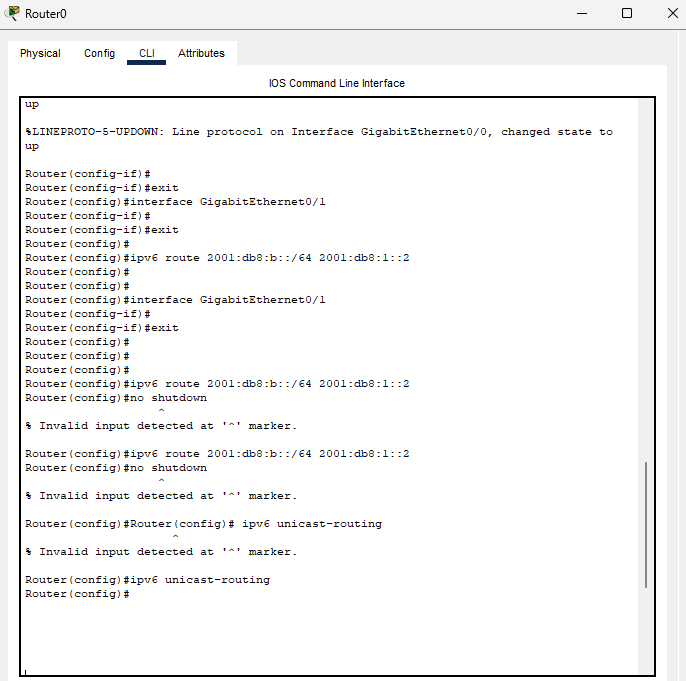
\includegraphics[width=0.8\textwidth]{P1/img/tumodsimulasi.png}
    \caption{Hasil simulasi}
    \label{fig:hasil_routing_ipv6}
    


\end{figure}

\begin{figure}
    \centering
    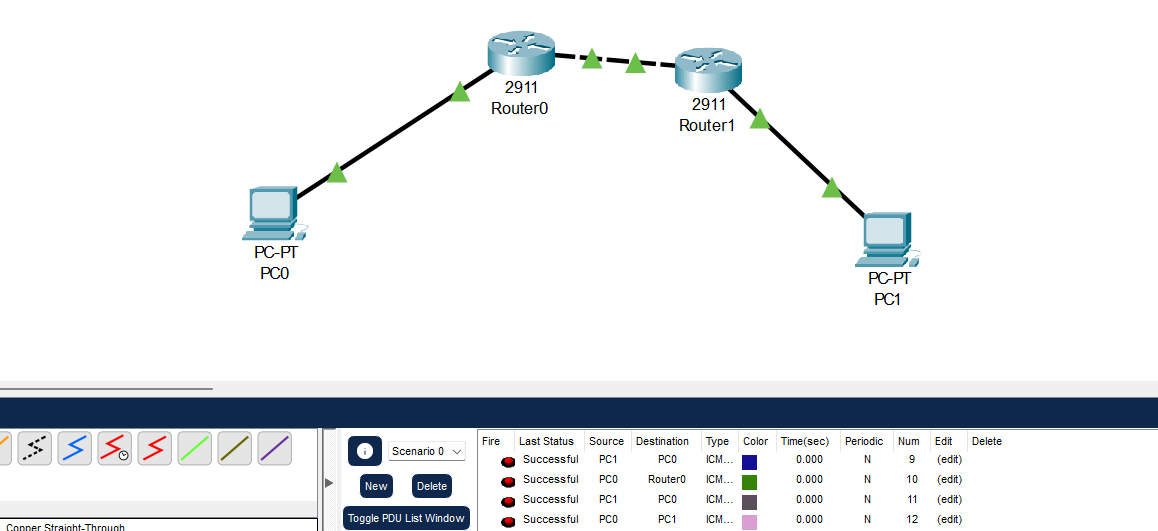
\includegraphics[width=0.8\textwidth]{P1/img/tumodsimulasi1.png}
    \caption{Hasil simulasi}
    \label{fig:hasil_simulasi_ipv6}
\end{figure}

\begin{figure}
    \centering
    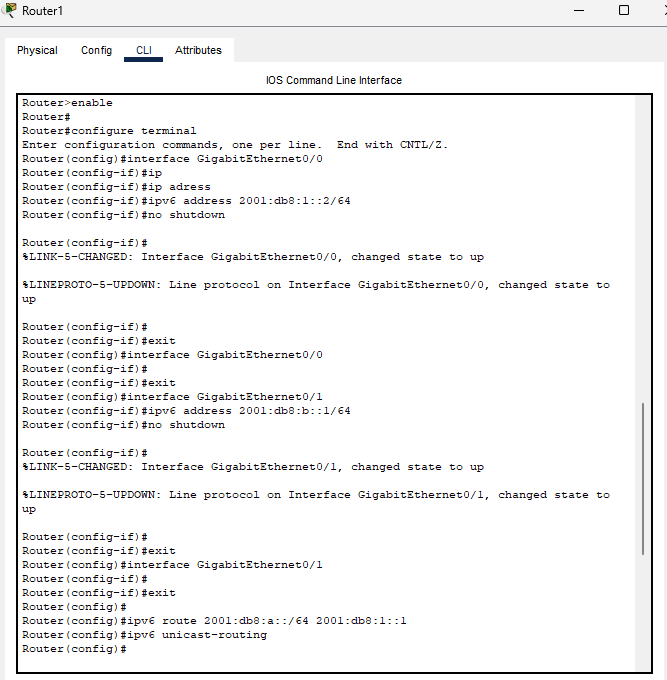
\includegraphics[width=0.8\textwidth]{P1/img/tumodsimulasi2.png}
    \caption{Hasil simulasi}
    \label{fig:hasil_routing_dinamis_ipv6}
\end{figure}

\begin{figure}
    \centering
    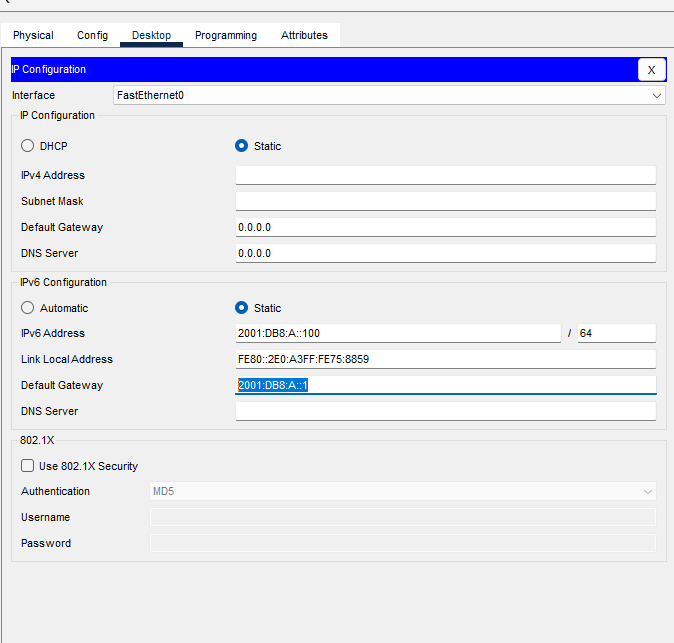
\includegraphics[width=0.8\textwidth]{P1/img/tumodsimulasi3.png}
    \caption{Hasil simulasi}
    \label{fig:hasil_uji_dinamis_ipv6}

\end{figure}

\begin{figure}
    \centering
    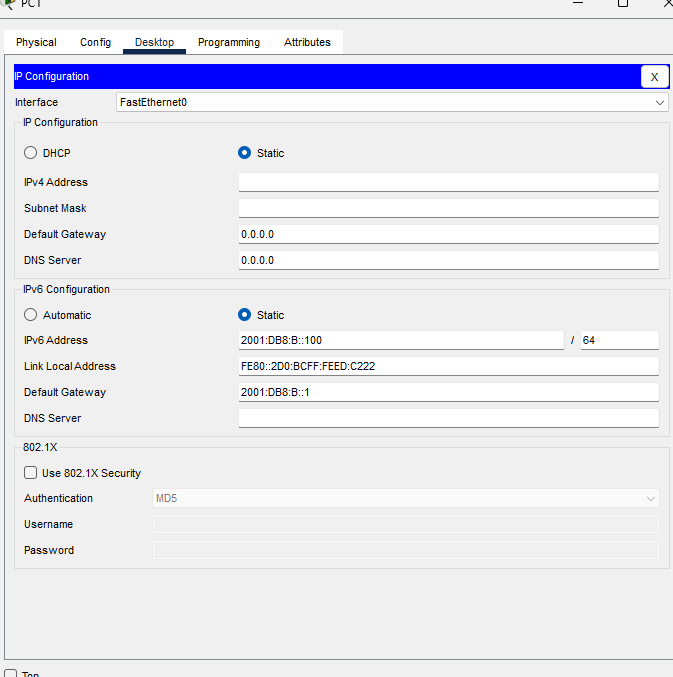
\includegraphics[width=0.8\textwidth]{P1/img/tumodsimulasip4.png}
    \caption{Hasil simulasi}
    \label{fig:hasil_routing_dinamis_ipv6_2}
\end{figure}


\section{Kesimpulan}Praktikum ini berhasil mendemonstrasikan implementasi routing statis IPv6, di mana konektivitas antar laptop yang terhubung ke router berbeda berhasil tercapai setelah konfigurasi alamat IP, gateway, dan rute statis dilakukan secara manual. Hal ini membuktikan bahwa pendekatan routing statis efektif untuk skenario jaringan yang telah ditentukan.

Di sisi lain, upaya untuk mengkonfigurasi routing dinamis IPv6 menggunakan OSPFv3 selama sesi praktikum di laboratorium mengalami kegagalan. Kendala ini, yang kemungkinan disebabkan oleh kesalahan dalam pengaturan instance OSPF, pemilihan interface, potensi masalah pada perangkat keras router, atau kurangnya pemahaman praktikan, mengakibatkan router tidak dapat membentuk hubungan neighbor dan bertukar informasi routing. Akibatnya, rute dinamis tidak muncul dan konektivitas antar jaringan lokal (LAN) tidak terwujud.

Namun, sebagai pelengkap, simulasi routing IPv6, baik statis maupun dinamis menggunakan RIPng, berhasil dilakukan melalui Cisco Packet Tracer. Ini memberikan wawasan tambahan mengenai konfigurasi dan operasional protokol routing dinamis dalam lingkungan yang terkontrol.

Secara keseluruhan, praktikum ini memberikan pemahaman praktis mengenai konfigurasi routing statis IPv6 yang sukses dan menyoroti tantangan serta kompleksitas dalam implementasi routing dinamis seperti OSPFv3 di lingkungan nyata. Pentingnya ketelitian dalam setiap langkah konfigurasi, pemahaman parameter protokol, dan kemampuan troubleshooting menjadi pembelajaran utama dari percobaan ini.
\section{Lampiran}
\subsection{Dokumentasi saat praktikum}
\begin{figure}
    \centering
    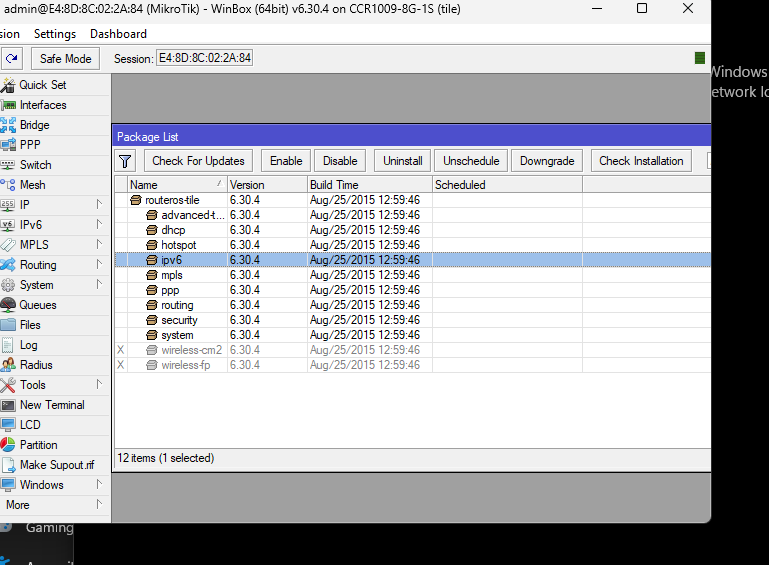
\includegraphics[width=0.8\textwidth]{P1/img/dokum1.png}
    \caption{Lampiran}
    \label{fig:hasil_routing_dinamis_ipv6_3}
\end{figure}
\begin{figure}
    \centering
    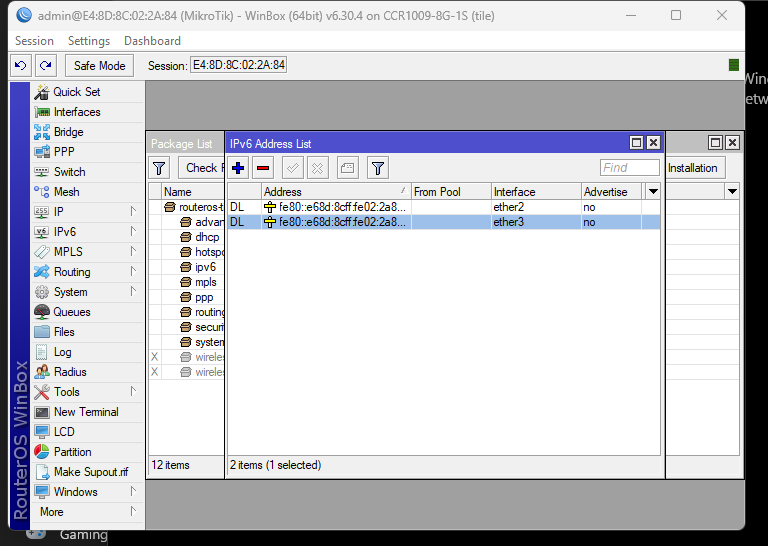
\includegraphics[width=0.8\textwidth]{P1/img/dokum2.png}
    \caption{Lampiran}
    \label{fig:hasil_routing_dinamis_ipv6_4}
\end{figure}
\begin{figure}
    \centering
    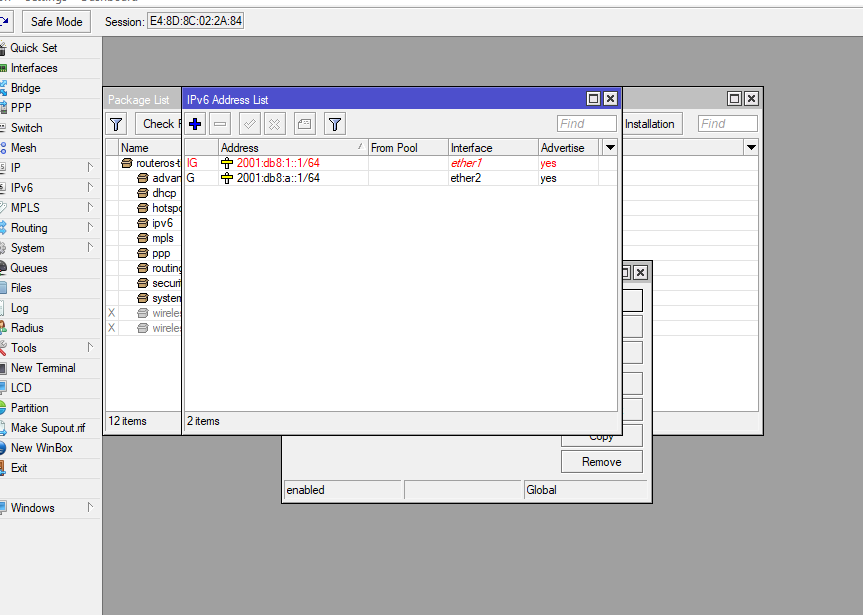
\includegraphics[width=0.8\textwidth]{P1/img/dokum3.png}
    \caption{Lampiran}
    \label{fig:hasil_routing_dinamis_ipv6_5}
\end{figure}
\begin{figure}
    \centering
    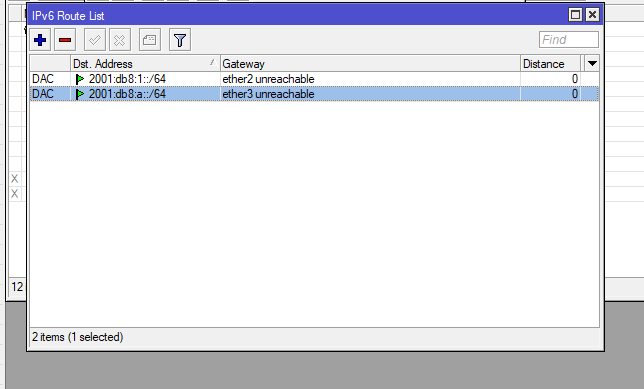
\includegraphics[width=0.8\textwidth]{P1/img/dokum4.png}
    \caption{Lampiran}
    \label{fig:hasil_routing_dinamis_ipv6_6}
\end{figure}
\begin{figure}
    \centering
    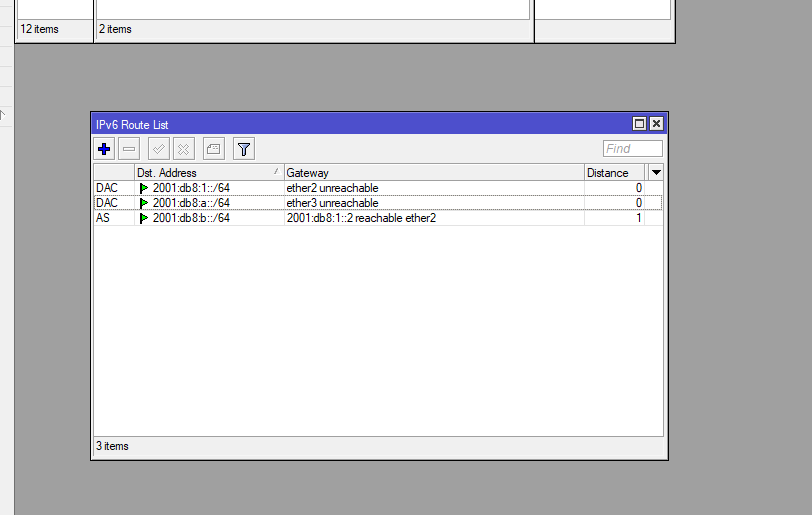
\includegraphics[width=0.8\textwidth]{P1/img/dokum5.png}
    \caption{Lampiran}
    \label{fig:hasil_routing_dinamis_ipv6_7}
\end{figure}